\section{Multivibratore astabile}
\begin{figure}[h]
	\centering
	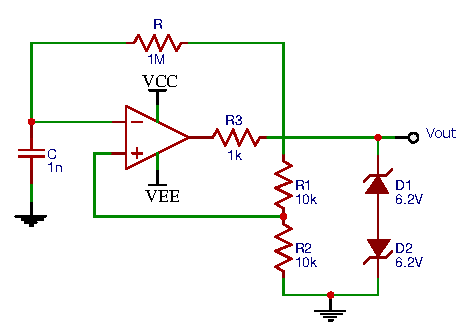
\includegraphics[scale=1]{circ_astabile.pdf}
	\caption{Circuito del multivibratore astabile utilizzato.}
	\label{f:multi_vibr}
\end{figure}
Si è montato il circuito in \fig{multi_vibr} e se ne sono misurati i valori dei componenti con il multimetro in \tab{misure_componenti}.
\begin{table}
	\centering
	\begin{tabular}{lc}
		& Misura \\
		\midrule
	$R$	&$\SI{972(8)}{\kohm}$\\
	 $R_1$	&$\SI{9.88(9)}{\kohm}$\\
	 $R_2$	&$\SI{9.88(9)}{\kohm}$\\
	 $R_3$	&$\SI{972(9)}{\ohm}$\\
	 $C$	&$\SI{1.04 \pm 0.07}{\nano\farad}$ \\
	\end{tabular}
	\caption{misure dei componenti del circuito}
	\label{t:misure_componenti}
\end{table}
I valori di $R$ e $C$ sono stati scelti in modo da avere un periodo di circa $\SI{2}{\ms}$ utilizzando la formula $T=2RC\log\frac{2+\frac{R_1}{R_2}}{\frac{R_1}{R_2}}$, dove T è proprio il periodo dell'onda quadra. Utilizzando l'oscilloscopio sono stati misurati i segnali nei punti $V_O , V_+ ,V_-$ come riportato nei grafici in \fig{stabile}, (\ref{f:astabile+}).
I valori ottenuti delle ampiezze dei tre segnali sono riportati in \tab{misure} insieme ai valori attesi.
I valori attesi sono $V_+=-V_-=\frac{V_\gamma +V_z}{1+\frac{R_1}{R_2}}$.  $V_O=\pm V_\gamma +V_z$ (il segno varia a seconda che sia il valore alto o basso), dove $V_\gamma$ e $V_z$ sono rispettivamente la tensione di polarizzazione diretta e la tensione di zener dei diodi (che assumiamo essere identici).
\begin{table}[h]
	\centering
	\begin{tabular}{lcccc}
	&Misurato [$\SI{}{\V}$]&Atteso [$\SI{}{\V}$] \\
	\midrule
	$V_O$	& $6.88(4)$	& $6.8$ \\
	$V_+$	& $3.48(2)$	& $3.4$ \\
	$V_-$	& $3.52(2)$	& $3.4$ \\
	\end{tabular}
	\caption{Ampiezze dei segnali misuarati e attesi.}
	\label{t:misure}
\end{table}

\begin{figure}[h]
	\centering
	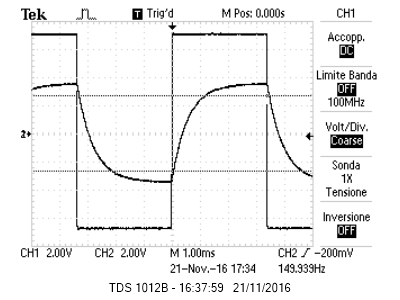
\includegraphics[scale=1]{astabile.png}
	\caption{L'nda quadra rappresenta $V_O$ mentre l'altra $V_-$.}
	\label{f:astabile}
\end{figure}

\begin{figure}[h]
	\centering
	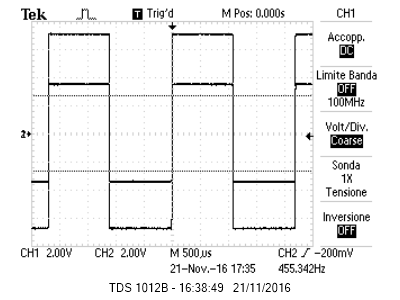
\includegraphics[scale=1]{astabilepiu.png}
	\caption{L'onda quadra di ampiezza maggiore è $V_O$ mentre l'altra è $V_+$}
	\label{f:astabile+}
\end{figure}

Il ruolo dei diodi zener è quello di limitare l'ampiezza della tensione in uscita in modo simmetrico tra $(V_\gamma + V_z)$ e $-(V_\gamma + V_z)$. Al comtempo si inserisce all'uscita dell'OpAmp la resistenza $R_3$ in modo da limitare la quantità di corrente che fluisce nei diodi zener e per permettere la caduta di tensione "in eccesso" rispetto a quella data dal clamping degli zener.


Come ci si può aspettare la frequenza i oscillazione non dipende dalla tensione di alimentazione. In effetti il periodo di oscillazione è previsto dalla formula già citata $T=2RC\log\frac{2+\frac{R_1}{R_2}}{\frac{R_1}{R_2}}$, che, appunto, non contiene dipendenze da $V_{cc}$ e $V_{ee}$.


Per quanto riguarda il comportamento ad alta frequenza si può vedere come l'onda quadra venga sostituita da una onda sinusoidale in \fig{freqzona}. Questo dovrebbe essere dovuto al comportamento a un polo dell'OpAmp ad alta frequenza, che, attenuando il segnale, causa un abbassamento dell'amplificazione. Ne risulta che l'OpAmp non va più in zona non lineare, ne si raggiunge la tensione di conduzione degli OpAmp(si vede come i due canali, uno su $V_O$, l'altro su $V_+$, siano quasi sovrapposti).

\begin{figure}[h]
	\centering
	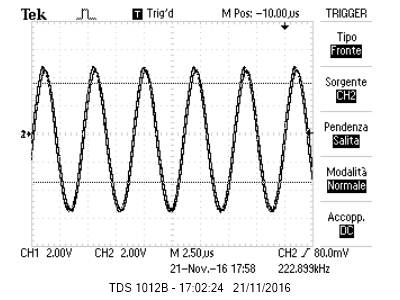
\includegraphics[scale=1]{astabilefrequenzona.png}
	\caption{Oscillatore astabile con frequenza di $\SI{220}{\mega\Hz}$}
	\label{f:freqzona}
\end{figure}
